\documentclass[line, margin]{res}

\usepackage{url}
\usepackage{hyperref}
\usepackage{graphicx}

\begin{document}
\name{Gurkirt Singh}
%\address{\textbf{Birth:} Jan'88\\ \textbf{Email:} \href{mailto:guru094@gmail.com}{\nolinkurl{guru094@gmail.com}}\\ \textbf{Webpage:} \url{https://sites.google.com/site/gurkirtcv/}}
\address{\textbf{Web:} \url{http://gurkirt.github.io/}\\\textbf{Email:} \href{mailto:gurkirt.singh-2015@brookes.ac.uk}{\nolinkurl{gurkirt.singh-2015@brookes.ac.uk}}\\\textbf{Tel:}+1 2368084391} 
%\address{\textbf{DOB:} Jan'88 \\ \textbf{Email:} \href{mailto:guru094@gmail.com}{\nolinkurl{guru094@gmail.com}}  %\textbf{Webpage:} \url{https://sites.google.com/site/gurkirtcv/}} }

\begin{resume}

%\begin{minipage}[c]{0.65\textwidth}
%\textbf{Contact Information:}\\
%T2.06, Wheatley Campus,\\
%Oxford Brookes University,\\
%Oxford, UK, OX33 1HX,\\
%Tel: +44-7424653155
%\end{minipage}
%\begin{minipage}[c]{0.55\textwidth}
%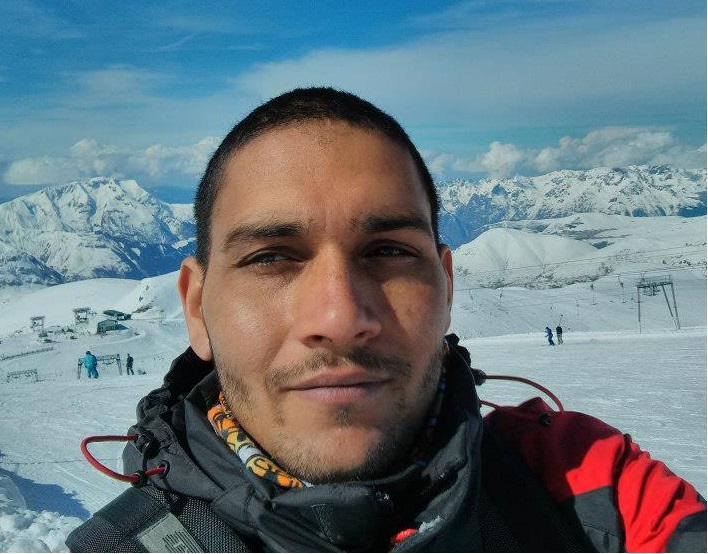
\includegraphics[width=.5\linewidth]{me.jpg}
%\end{minipage}
%\noindent
%\parbox{8cm}{}
%\hfill

\section{Interests}
Computer Vision and Machine learning


\section{Education} 
\textbf{PhD} in Computing and Maths  \hfill Sept'15 - present \quad  Expected submission: July 2019\\
\href{http://cct.brookes.ac.uk/research/isec/artificial-intelligence/index.html}{\textbf{Artificial Intelligence and Vision research group}}, Oxford Brookes University\\
Proposed thesis direction: \emph{Online action detection and prediction in videos.} \\
Supervisors: 
%\href{http://cms.brookes.ac.uk/staff/FabioCuzzolin/}
{Professor Fabio Cuzzolin}

\textbf{Research Master}, Specialization: \emph{Graphics Vision and Robotics} \hfill 2012 - 2013\\
\href{http://ensimag.grenoble-inp.fr/}{\textbf{ENSIMAG - Grenoble INP, France}}\\
Grades: 13.74/20.00  \  \ Max Grades in class: 16.12/20.00\\
Thesis: \emph{Frame-wise representations of depth videos for action recognition.} 
Supervisors: Professor. Radu Horaud and Dr. Georgios Evangelidis
%%Supervisors: \href{https://team.inria.fr/perception/team-members/radu-patrice-horaud/}{Dr. Radu Patrice HORAUD} and \href{https://team.inria.fr/perception/team-members/evangelidis/}{Dr. Georgios EVANGELIDIS}

\textbf{B.Tech.} in \textbf{Electronics and Instrumentation Engineering.} \hfill 2006 - 2010\\
\href{http://www.vit.ac.in/}{VIT University, Vellore, India}; 
CGPA: 8.33/10.00 \\%%\  \ Max CGPA in class: 9.69/10.00 \\
Thesis: 
%\emph{\href{http://homepages.inf.ed.ac.uk/rbf/FORUMTRACKING/SINGH/GurkirtSingh.pdf}
\emph{Categorising the Abnormal Behaviour from an Indoor Overhead Camera.}\\
Supervisor: %\href{http://homepages.inf.ed.ac.uk/rbf/}
{Professor Bob Fisher} from University of Edinburgh, UK
%%Supervisor: \href{http://homepages.inf.ed.ac.uk/rbf/}{Dr. Bob Fisher} 

\section{Contests}
Charades-2017: Acton Recognition and Segmentation tasks (Rank: \textbf{2}/10 and 3/6) \hfill 2016\\
ActivityNet-2017: Classification tasks (Rank 3/29)  \hfill 2016\\
ActivityNet-2016: Classification and Detection tasks (Rank 10/24 and \textbf{2}/6) \hfill 2016\\
Chalearn Looking at People Challenge (Gesture Detection Task Rank 7/17) \hfill 2014\\
Chalearn Multi-Modal Gesture Recognition Challenge (Rank 17/54) \hfill 2013

\section{Recent \ Experiences}
\textbf{BorealisAI, Vancouver, Canada} \hfill Feb'19 - May'19 \\
Research Intern, Computer Vision\\
\emph{Human Object Interaction Detection in Videos.}\\
Supervisors: Leonid Sigal and Greg Mori 

\textbf{Disney Research Pittsburgh, USA} \hfill Feb'17 - July'17 \\
Research Intern, Computer Vision\\
\emph{Temporal Activity Detection in untrimmed videos of TV-episodes.}\\
Supervisors: Leonid Sigal and Andreas Lehrmann 

\textbf{Siemens Corporate Research and Technology, India} \hfill Oct'13 - Aug'15 \\
Research Engineer, Imaging and Computer Vision group\\
\emph{Multiple Object detection and tracking for video surveillance applications}\\
Collaborator: Siemens Corporate Research, Princeton, USA 

%\href{https://team.inria.fr/perception/}
\textbf{Perception team, INRIA Grenoble, France}  \\
Research Engineer: %\href{http://gesture.chalearn.org/2013-multi-modal-challenge}
{\emph{Multi-modal gesture recognition.}} \hfill June'13 - Sept'13 \\
Master thesis:\emph{Frame-wise representations of depth videos.} \hfill Jan'13 - May'13 \\
Supervisors: Dr. Georgios Evangelidis and Dr. Radu Horaud 

%\textbf{\href{http://www.ed.ac.uk/home}
\textbf{University of Edinburgh, UK} \hfill Jan'10 - May'10 \\
Intern at %\href{http://wcms.inf.ed.ac.uk/ipab/}
{Institute of Perception, Action and Behaviour} \\ 
Title: \emph{Categorising the Abnormal Behaviour from an Indoor Overhead Camera.} \\
Supervisor:
%\href{http://homepages.inf.ed.ac.uk/rbf/}
{Dr. Bob Fisher} 

%\textbf{\href{http://www.iitd.ac.in/}
\textbf{Vision and Graphics lab IIT Delhi, India} \hfill May'11 - March'12 \\
Project Associate, \emph{Implementation of Interactive Single View Image Based Model Reconstruction.} AND. 
\emph{Moving object detection with moving camera.} \\
Supervisors: Dr. Subhashis Banerjee

%\textbf{\href{http://www.iitk.ac.in/}
\textbf{SMSS lab, IIT Kanpur, India} \hfill June'10 - March'11 \\
Project Associate, \emph{Control of Reconfigurable Parabolic Antenna using SMA actuators.}\\
Supervisors: Dr. Bishakh Bhattacharya\\


\section{Selected Publications} 
\textbf{Gurkirt Singh} and Fabio Cuzzolin, 
\emph{Recurrence to the Rescue: Towards Causal Spatiotemporal Representations}, 
arXiv: 1811.07157 (2018).

\textbf{Gurkirt Singh}, Suman Saha and Fabio Cuzzolin, 
\emph{Predicting Action Tubes}, in AHB2018 workshop at ECCV  2018. \textbf{3} citations.

\textbf{Gurkirt Singh}, Suman Saha and Fabio Cuzzolin, 
\emph{TraMNet - Transition Matrix Network for Efficient Action Tube Proposals}, 
ACCV, Perth, 2018.

\textbf{Gurkirt Singh}${}^*$, Stephen Akrigg${}^*$, Valentina Fontana${}^*$, 
Manuele Di Maio, Suman Saha, Fabio Cuzzolin, 
\emph{Action Detection from a Robot-Car Perspective }, 
preprint arXiv: 1807.11332 ${}^*$ means equal contribution

\textbf{Gurkirt Singh}, Suman Saha, Michael Sapienza, Philip Torr and Fabio Cuzzolin, 
\emph{Online Real-time Multiple Spatiotemporal Action Localisation and Prediction}, 
ICCV, 2017. \textbf{67} citations.

Suman Saha, \textbf{Gurkirt Singh} and Fabio Cuzzolin, 
\emph{AMTnet: Action-Micro-Tube Regression by end-to-end Trainable Deep Architecture}, 
ICCV, 2017. \textbf{22} citations.

Harkirat Behl, Michael Sapienza \textbf{Gurkirt Singh}, Suman Saha, Fabio Cuzzolin and Philip Torr,
\emph{Incremental Tube Construction for Human Action Detection},
BMVC, 2018. \textbf{3} citations.

% Suman Saha, \textbf{Gurkirt Singh}, Michael Sapienza, Philip Torr and Fabio Cuzzolin, 
% \emph{Spatio-temporal human action localisation and instance segmentation in temporally untrimmed videos}, arXiv, 2017. 

Suman Saha, \textbf{Gurkirt Singh}, Michael Sapienza, Philip Torr and Fabio Cuzzolin, 
\emph{Deep Learning for Detecting Multiple Space-Time Action Tubes in Videos}, 
in BMVC 2016, \textbf{83} citations.

\textbf{Gurkirt Singh} and Fabio Cuzzolin, 
\emph{Untrimmed Video Classification for Activity Detection: Submission to ActivityNet Challenge}, 
arXiv: 1607.01979 (2016), \textbf{2nd} position in Activity Detection challenge at ActivityNet workshop CVPR 2016, \textbf{36} citations.

Georgios Evangelidis, \textbf{Gurkirt Singh}, Radu Horaud, 
%\href{https://sites.google.com/site/gurkirtcv/research/continuous}
\emph{Continuous Gesture Recognition from Articulated Poses}, 
in ChalearnLAP2014 workshop at ECCV  2014. \textbf{37} citations.

%This work was carried out in context of in Multi-modal gesture recognition challenge 2014. Our team ranked 8th out of 17 by using only Skeleton information.\\
%Keywords: gesture detection, dynamic programming, skeleton descriptor
Georgios Evangelidis, \textbf{Gurkirt Singh}, Radu Horaud,
%\href{https://team.inria.fr/perception/research/icpr2014/}
\emph{Skeletal Quads: Human action recognition using joint quadruples}, 
in ICPR 2014 Stockholm. \textbf{182} citations.
%We propose a local skeleton descriptor that encodes the relative position of joint quadruples. Such a coding implies a similarity normalisation transform that leads to a compact (6D) view-invariant skeletal feature. 
%Further, the use of a Fisher kernel representation is suggested to describe the skeletal quads contained in a action. \\
%Keywords: multi-level Fisher vectors, linear SVM
%\section{THESIS}
%\textbf{Gurkirt Singh} and Georgios Evangelidis, {\emph{Participated in Multi-modal gesture recognition 2013 using RGB-D, Skeleton and Audio}}, 
%\href{http://gesture.chalearn.org/2013-multi-modal-challenge}
%11th out of 17 by using alone Skeleton information.
%We build a BOW representation of using skeleton-quad  descriptors from human joint positions. Dynamic programming was used for simultaneous recognition and segmentation of gestures. \\

\textbf{Master's thesis}, \href{https://sites.google.com/site/gurkirtcv/research/master-thesis}{\emph{Frame-wise Representations of Depth Videos for Action Recognition.}}\\
We investigate the of problem continuous action recognition from depth images. 
Three types of depth frame data representation are proposed. 
Further, we investigate the frame-wise classification as a solution for the continuous action detection problem.

\textbf{Bachelor's thesis} \href{https://sites.google.com/site/gurkirtcv/research/btechproject}{\emph{Categorising the Abnormal Behaviour from an Indoor Overhead Camera.}}
We propose an approach of using an overhead camera to detect the anomalous events based on the trajectories of moving objects with and EER (Equal Error rate) of only 1.2\%. I contributed 65000 trajectories to \href{http://homepages.inf.ed.ac.uk/rbf/FORUMTRACKING/}{\emph{Edinburgh Informatics Forum Pedestrian Database}}.

\section{Skills}
\textbf{Programming: } Python, Matlab, C/C++, Lua.\\
\textbf{Deep Learning Platforms:} PyTorch, Torch, Caffe. \\
\textbf{Libraries:} OpenCV, Eigen, Scikit-Learn, Numpy, Scipy, Kinect SDK.\\
\textbf{Operating Systems:} Linux and Windows.\\
\textbf{Development Environments:} VS code, Eclipse, Spyder, Pycharm.

\section{Languages}
Punjabi (Maternal), Hindi (Fluent), English (Fluent), French (Elementary)\\

\section{REFEREES}
\href{http://cms.brookes.ac.uk/staff/FabioCuzzolin/}{Professor Fabio Cuzzolin}, Oxford Brookes University, UK.\\
\href{http://www.robots.ox.ac.uk/~phst/}{Professor Philip Torr}, University of Oxford, UK.\\
\href{https://www.cs.ubc.ca/~lsigal/}{Professor Leonid Sigal}, University of British Columbia, Canada.\\
\href{https://ps.is.tuebingen.mpg.de/person/alehrmann}{Dr. Andreas Lehrmann}, Disney Research Pittsburgh, USA.\\
\href{http://homepages.inf.ed.ac.uk/rbf/}{Professor Bob Fisher}, University of Edinburgh, UK.\\
%\href{https://team.inria.fr/perception/team-members/radu-patrice-horaud/}{Professor Radu Patrice HORAUD}, INRIA, Grenoble, France.\\
\href{https://team.inria.fr/perception/team-members/evangelidis/}{Dr. Georgios EVANGELIDIS}; Daqri, USA.\\
\href{http://www.cfar.umd.edu/~kale/}{Dr. Amit Kale}, Bosch Research, India.

%\section{MISC}
%Attended International Computer Vision Summer school, Sicili, 2016, was part of winning reading group.
\end{resume}
\end{document}